% Supplementary Material for:
% Recursive prototyping for computational behavior analysis from egocentric videos
%
\documentclass[runningheads]{llncs}

\usepackage[T1]{fontenc}
\usepackage{graphicx}
\usepackage{booktabs}
\usepackage{amsmath}
\usepackage{amssymb}
\usepackage{bbm}
\usepackage{cleveref}
\usepackage{url}
\usepackage{multirow}

\begin{document}

\title{Supplementary Material: Recursive prototyping for computational behavior analysis from egocentric videos}

\titlerunning{Supplementary Material}

\author{Sam Perochon\inst{1, 2}\orcidID{0000-0002-1759-4154} \and
Laurent Oudre\inst{1, 2}\orcidID{0000-0002-4750-2265}}

\authorrunning{S. Perochon and L. Oudre}

\institute{Universit\'e Paris Saclay, Universit\'e Paris Cit\'e, ENS Paris Saclay, CNRS, SSA, INSERM, Centre Borelli, F-91190, Gif-sur-Yvette, France \and
Service Neurologie, AP-HP, H\^opital National d'Instruction des Arm\'ees, F-92140, Clamart, France}

\maketitle

% \tableofcontents


%==============================================================================
\section{Clustering behavior across vocabulary sizes}
\label{sec:supp_clustering_motivation}
%==============================================================================

To illustrate the underlying clustering challenge and motivate our recursive approach, we define naive prototypes as the centroids estimated using cosine $k$-means clustering on all available VideoMAE-v2 embeddings for increasing vocabulary size $G$. We visualize the resulting symbolic representations in \Cref{fig:supp_assignments_across_K}.

\begin{figure}[!htbp]
    \centering
    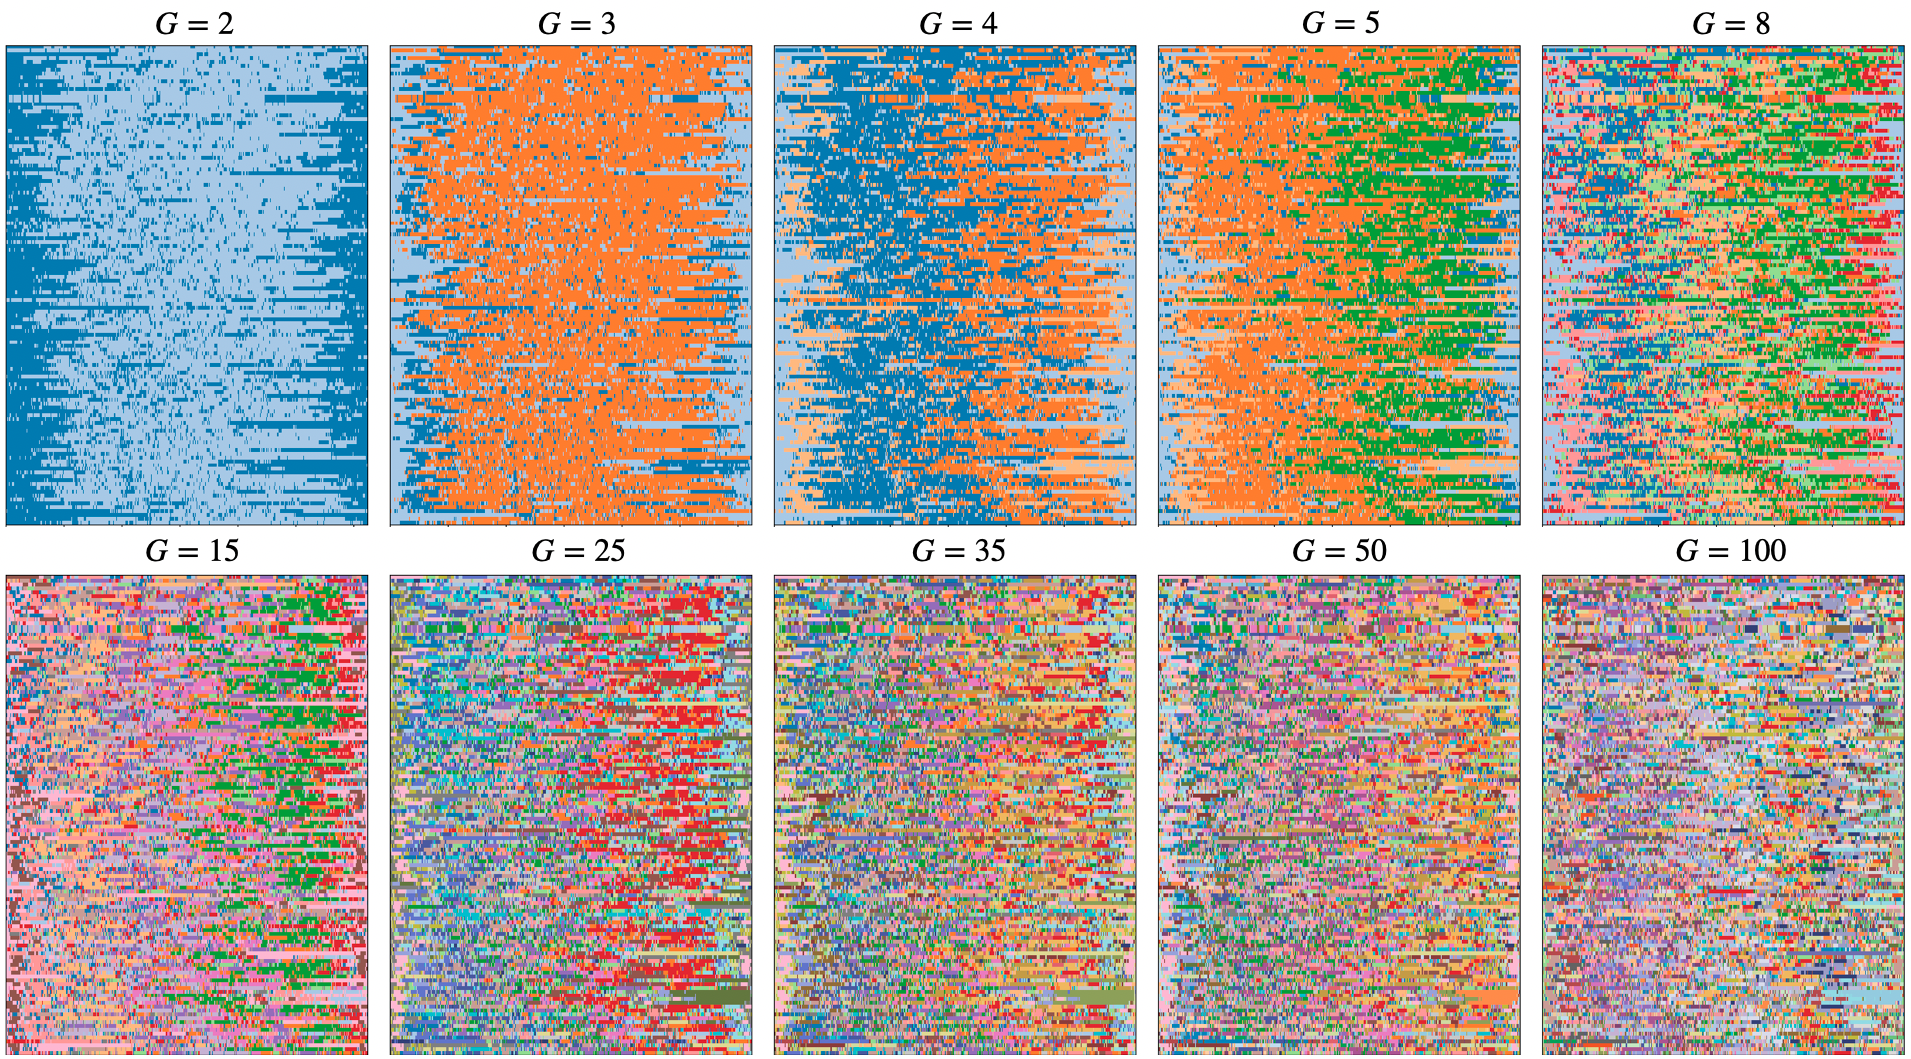
\includegraphics[width=1.0\linewidth]{figures/chapter_5_assignements_across_K.png}
    \caption{\textbf{Participant's symbolic representation for increasing vocabulary size.} Each row corresponds to a different participant performing the cooking task, and each color represents a different cluster. Sequences are upsampled to match the longest sequence for visualization purposes. Coarse clusters reveal inter-subjects temporal consistency, while finer clusters capture more specific visual atoms.}
    \label{fig:supp_assignments_across_K}
\end{figure}

We observe a remarkable temporal consistency of prototype assignments across participants, especially for low $G$, suggesting the feasibility of learning a generalizable vocabulary. To relate these clusters to the structure of participants' similarity matrices, we compute and visualize in \Cref{fig:supp_gram_participants} the cosine similarity matrices of six participants from the control and patient groups.

\begin{figure}[!htbp]
    \centering
    \includegraphics[width=1.0\linewidth]{figures/gram_participant_raw.png}
    \caption{\textbf{Pairwise cosine similarity matrix between time-aligned embeddings for three control participants (top) and three patients with radiation-induced leukoencephalopathy (RIL) (bottom).} The color scale represents the cosine similarity between pairs of latent embeddings, with warmer colors indicating higher similarity. Key steps can be identified, such as reading the recipe (purple bar on the left) and breaking the eggs (orange bar). Our prototyping approach focuses on the smallest diagonal blocks of stable elevated similarity.}
    \label{fig:supp_gram_participants}
\end{figure}

The organization of participants' visual trajectory combines (i) short sequential atomic actions at fine granularity, and (ii) hierarchical patterns emerging within larger diagonal blocks. Coarse prototypes (low $G$) correspond to large-scale diagonal blocks merging several atomic visual atoms, while finer-grained prototypes (high $G$) more likely capture specific and unequivocal visual atoms.

However, in our high-dimensional ($D=1408$) and high-complexity setting (e.g., $K\in [10^2, 10^3]$), direct clustering of the empirical sample ($N \approx 906k$)---sometimes referred to as the extreme clustering setting \cite{10.1145/3097983.3098079}---does not readily produce a reliable vocabulary, due to clusters emerging at variable scales. This observation motivates our recursive latent subspace exploration procedure.

%==============================================================================
\section{Detailed centroids accumulation algorithm}
\label{sec:supp_algorithm}
%==============================================================================

Let $X_{\text{train}} = \{ x_1, ..., x_N \} \in (\mathbb{R}^{D})^N$ denote a set of $N$ training latent embeddings. The centroid accumulation stage proceeds iteratively over $P$ steps. At each step $p \geq 1$, the following operations are performed:

\begin{enumerate}
    \item \textbf{Generative step.}
    Estimate $C$ candidate centroids $\mu^{p} = (\mu^p_1, ..., \mu^p_C) \in \mathbb{R}^D$ by applying cosine $k$-means clustering to the residual set $R_p$. The centroids are estimated by solving:
    \begin{equation}
        \hat{\mu}^p = \arg \min_{\mu^p_{1},\dots,\mu^p_{C}} \;
        \sum_{x_i \in R_p} \Bigl(1 - \tfrac{x_i^\top \mu^p_{c_i}}{\|x_i\|\;\|\mu^p_{c_i}\|}\Bigr),
    \label{eq:supp_kmeans_objective}
    \end{equation}
    where $c_i \in [C]$ is the cluster assignment of $x_i$, defined as $c_i = \arg \min_{c \in [C]} \bigl(1 - \tfrac{x_i^\top \mu^p_{c}}{\|x_i\|\;\|\mu^p_{c}\|}\bigr)$.

    \item \textbf{Discriminative step.}
    Each of the $C$ empirical clusters is manually reviewed using the annotation protocol (see \Cref{sec:supp_annotation_protocol}), separating centroids into two disjoint subsets:
    \begin{itemize}
        \item $I_p^+ \subset [C]$: centroids associated with fine-grained and unequivocal clusters.
        \item $I_p^- = [C] \setminus I_p^+$: centroids associated with semantically ambiguous clusters.
    \end{itemize}
    We denote $A_p = \bigcup_{k=1}^p \{ \mu^k_j\}_{j\in I_k^+}$ the set of accumulated centroids up to step $p$, and $N_p = \{ \mu^p_c \}_{c \in I_p^-}$ the set of rejected centroids.

    \item \textbf{Samples assignments update.} Sample assignments are updated using centroids from $A_p \cup N_p$. We denote $d_i = \min_{c \in A_p \cup N_p} d(x_i, \mu_c)$ the assignment distance of sample $x_i$ to its closest centroid.

    \item \textbf{Residual set update.} The residual set $R_{p+1}$ is defined from two sources:
    \begin{itemize}
        \item Samples associated with the ambiguous subset of centroids $N_p$.
        \item Samples associated with valid centroids in $A_p$ whose assignment distance exceeds a centroid-specific threshold $d^{\text{min}}_c$.
    \end{itemize}
    The initial residual set comprises all samples: $R_1 = X_{\text{train}}$.
\end{enumerate}

The procedure ends at step $P$ when the accumulated number of source prototypes exceeds a predefined number $K_{\text{max}}$, yielding a set of $K$ prototypes $\mu^{[K]} = A_P = (\mu_1, ..., \mu_K)$.

\paragraph{Implementation notes.}
We use cosine $k$-means implemented in the \texttt{Faiss} library \cite{douze2024faiss}, which was found in preliminary experiments to maximize the number of retained clusters in the first round compared to other implementations and distance metrics. A constant threshold $d_c^{\text{min}}=0.3$ is used for all accepted centroids, corresponding approximately to the first quartile of assignment distance values. Annotations are collected using \texttt{pigeon-annotation}. Confidence intervals for NMI and ARI are computed via 1,000 bootstrap resamples.

%==============================================================================
\section{Analysis of the residual space definition}
\label{sec:supp_residual_thresholding}
%==============================================================================

The residual set at each iteration $p$ is designed to contain embeddings whose semantics are not yet captured by the current accumulated centroids. Samples are included in the residual set if their assignment distance exceeds a threshold $d_{\min}^k$. We evaluated several thresholding strategies:

\begin{itemize}
    \item $d_{\min}^k = Q_1(d_k)$: first quartile of cluster $k$ assignment distances
    \item $d_{\min}^k = Q_2(d_k)$: median of cluster $k$ assignment distances
    \item $d_{\min}^k = \text{mean}(d_k) + \text{std}(d_k)$: one standard deviation above mean
    \item $d_{\min}^k = \text{mean}(d_k) + 2\cdot\text{std}(d_k)$: two standard deviations above mean
    \item $d_{\min} \in [0.05, 1]$: fixed distance threshold
\end{itemize}

\Cref{fig:supp_residual_threshold} shows the evolution of residual set size across iterations for different thresholding strategies.

\begin{figure}[!htbp]
    \centering
    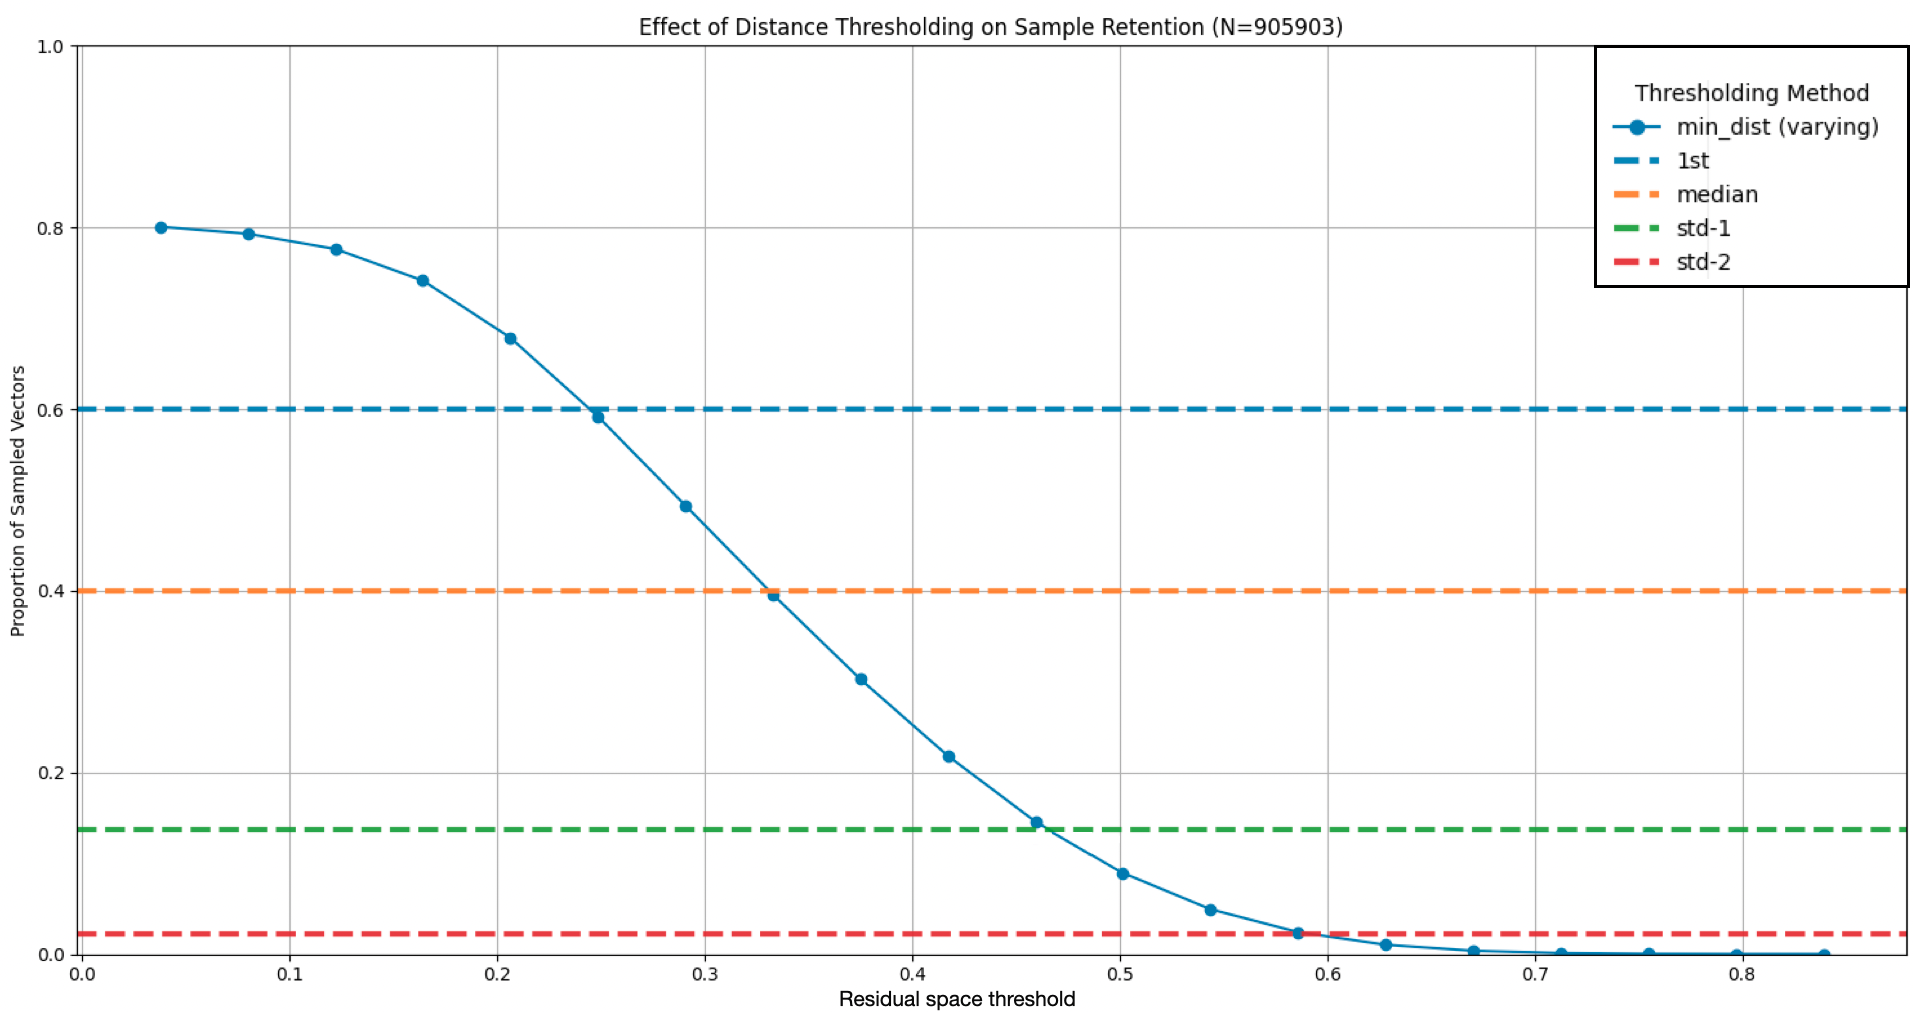
\includegraphics[width=0.9\linewidth]{figures/chapter_5_resildual_space_threshold.png}
    \caption{\textbf{Percentage of samples in the residual space across thresholding strategies.} Different curves correspond to fixed thresholds (first quartile, median) and adaptive thresholds based on cluster-specific assignment distance distributions. The fixed threshold $d_{\min}=0.3$ (approximately first quartile) provides a reasonable trade-off between retaining sufficient samples for subsequent iterations and ensuring accepted centroids have high-confidence assignments.}
    \label{fig:supp_residual_threshold}
\end{figure}


%==============================================================================
\section{Extended analysis of the annotation protocol}
\label{sec:supp_annotation_protocol}
%==============================================================================

Recovering the clusters interpretability is crucial for ensuring meaningful interpretations of the symbolic representations in downstream analysis tasks. We introduce a \emph{Visual Probing Mechanism} (VPM) to identify semantically consistent clusters and filter out ambiguous ones. 

The assignment distance associated with each sample can be used to rank empirical samples within each cluster, which we leverage to formulate the following hypotheses:  
\begin{itemize}
    \item \textbf{H1:} Cluster semantics can be recovered by inspecting a large number of independent samples drawn from the nearest neighbors of their centroid.
    \item \textbf{H2:} Cluster semantic consistency can be evaluated by inspecting a large number of independent samples drawn from their most distant assigned elements.
    \item \textbf{H3:} Visual inspection of the central frame of an embedding input sequence conveys sufficient information to recover its semantics.
\end{itemize}
While \textbf{H1} focuses on recovering the underlying semantics of clusters and assessing their granularity, \textbf{H2} aims to probe worst-case assignments to verify semantic consistency relative to the nearest samples. In particular, in the absence of supervised labels, these distant samples can serve as a proxy to assess data-fitting performance, as discussed in the manuscript. In practice, we observed that inspecting the closest and furthest neighbors for $30$ different participants appear sufficient to validate \textbf{H1} and \textbf{H2}, as discussed below. 

\subsection{Analysis of nearest-neighbors to recover clusters semantics and filter out ambiguous clusters (H1)}

Illustrative examples of accepted and rejected clusters are shown in \Cref{fig:chapter_5_definitive_examples} and \Cref{fig:chapter_5_ambiguous_examples}, respectively. Accepted clusters correspond to highly consistent participant actions, supporting the hypothesis that the proposed VPM can be used to reliably assess the action semantics of clusters, which ultimately map to behavior. In contrast, \Cref{fig:chapter_5_ambiguous_examples} shows several ambiguous clusters that were rejected during the annotation process and are intended for refinement in later stages of the procedure.

\begin{figure}[!htbp]
    \centering
    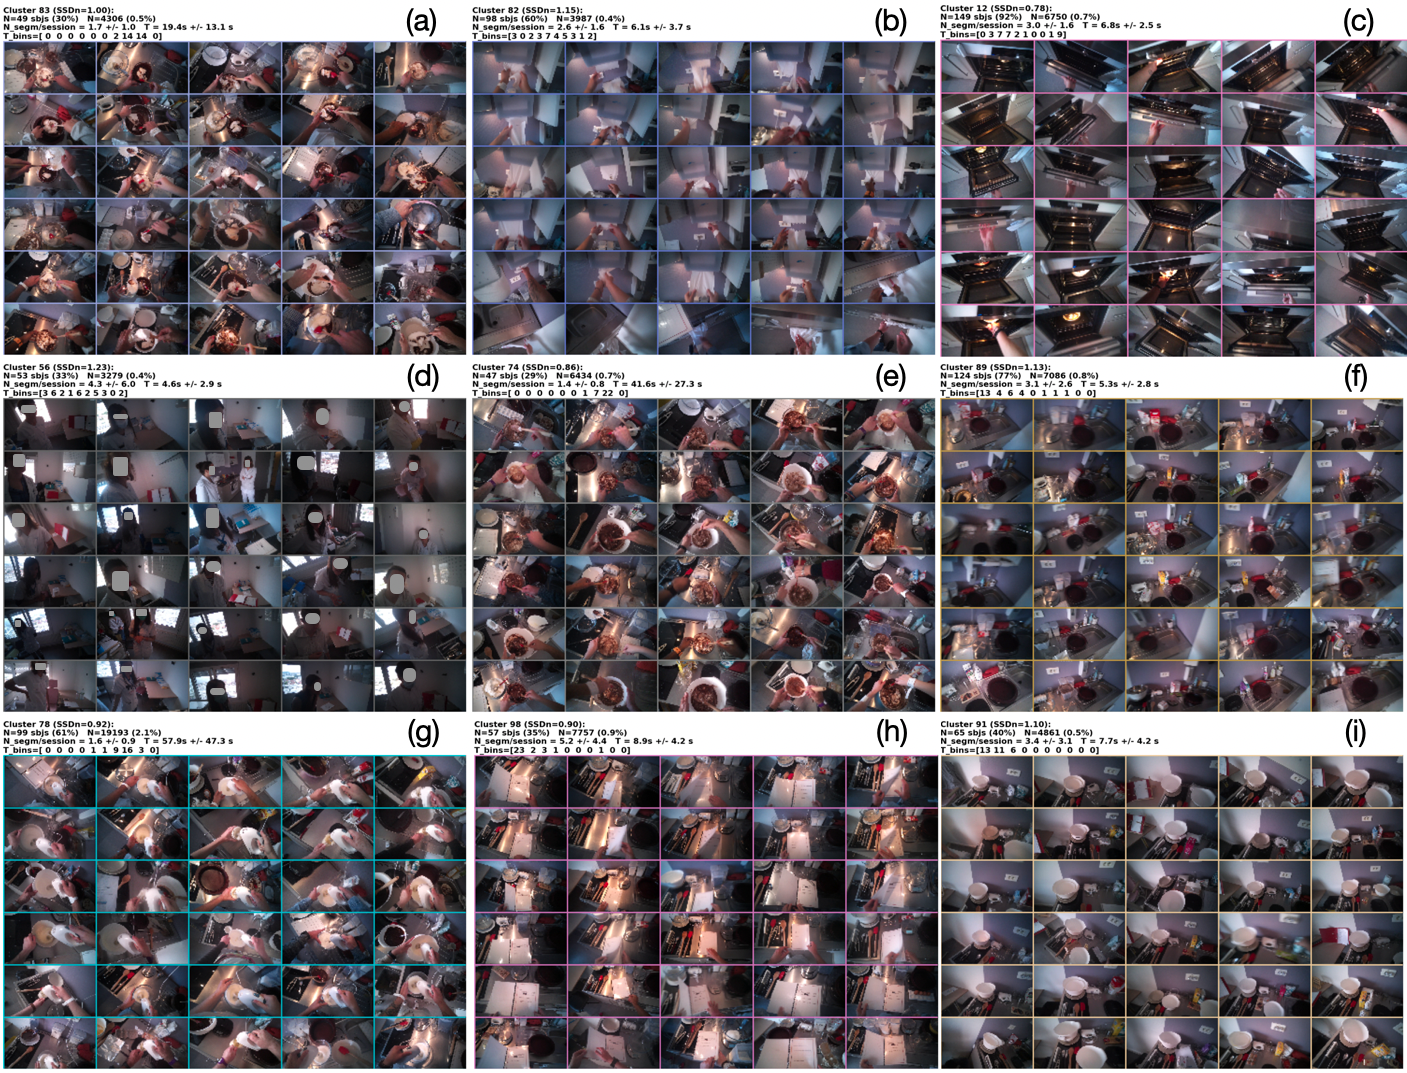
\includegraphics[width=1.0\linewidth]{figures/chapter_5_definitive_examples.png}
    \caption{\textbf{Illustrative examples of nearest-neighbors visual probes for nine accepted clusters.} Each subplot shows 30 independent occurrences of a given cluster, sampled from its most strongly associated nearest samples. These examples exhibit a high level of visual consistency across participants. The actions underlying each cluster can be identified unequivocally and robustly from their visual signatures. For example, (a) encodes ``adding flour to the dough'' and mostly occurs towards the end of the assessment; (b) encodes ``pulling a paper'' and seems temporally uniformly distributed; (c) ``opening the oven''; (d) ``talking to the clinician''; (e) ``mixing the dough''; (f) ``looking at the sink''; (g) ``using the mixer''; (h) ``reading the recipe''; and (i) ``looking at the material''. We add for each cluster their (a) average assignment distance; (b) sum-of-squared cosine distance (SSD) normalized by the total SSD; (c, d) prevalence across subjects and embeddings; (e) average (s.t.d) number of segment occurrences across participants; (f) average (s.t.d.) segment duration across participants; and (g) the distribution of normalized timestamps of the drawn samples across ten equally-sized temporal bins.}
    \label{fig:chapter_5_definitive_examples}
\end{figure}

\begin{figure}[!htbp]
    \centering
    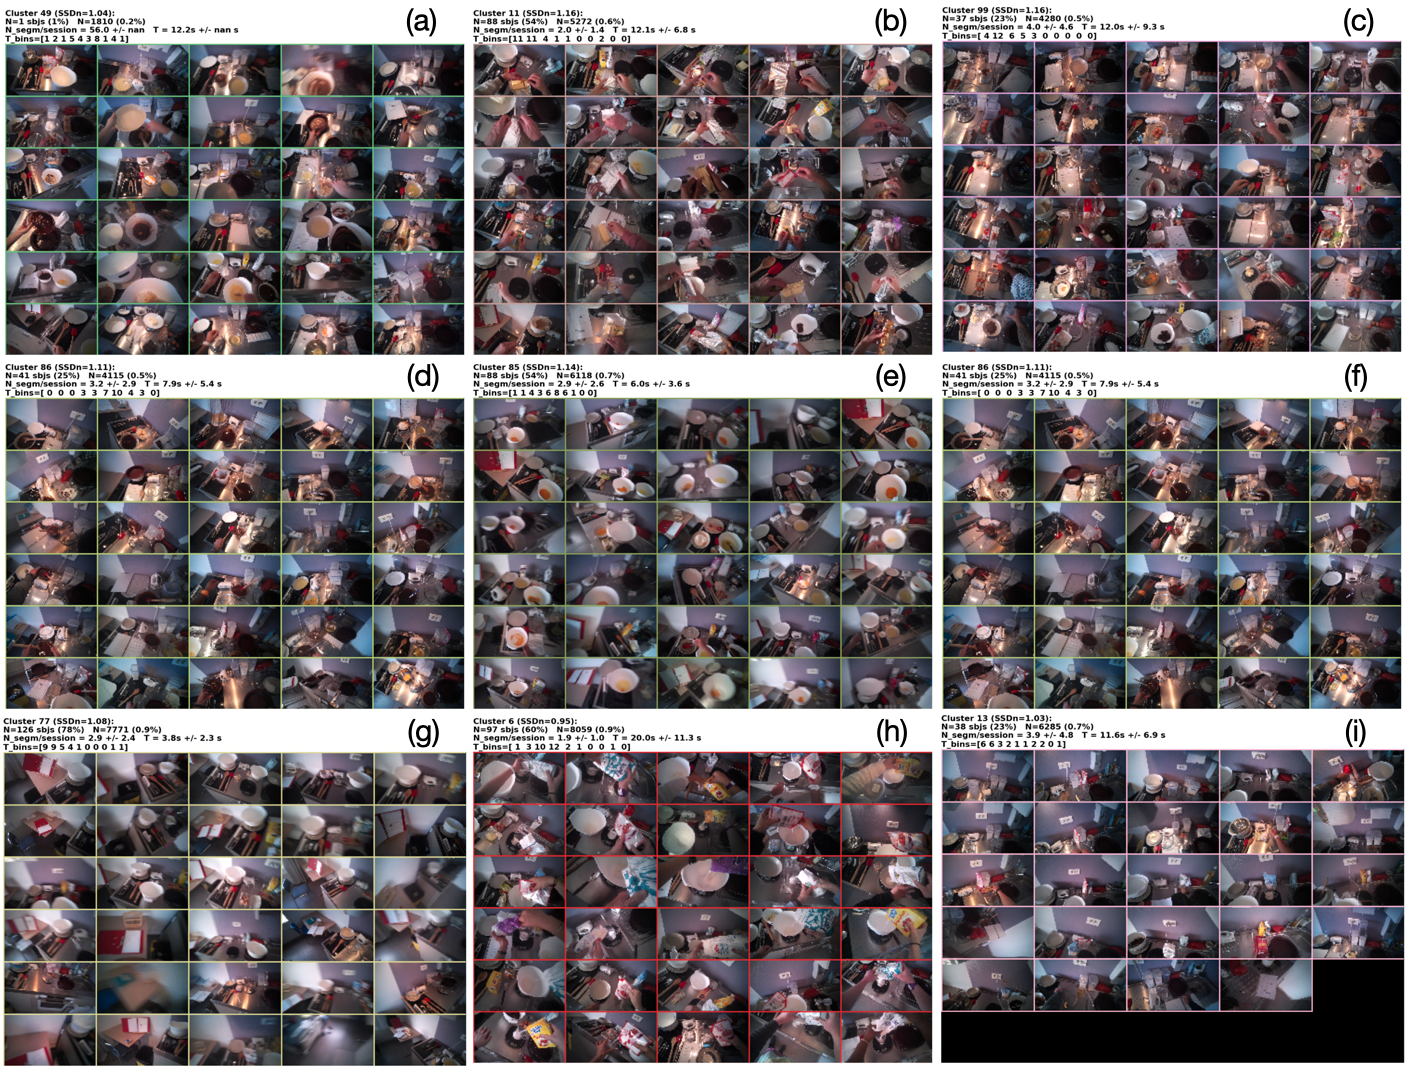
\includegraphics[width=1.0\linewidth]{figures/chapter_5_ambiguous_examples.png}
    \caption{\textbf{Illustrative examples of nearest-neighbor visual probes for nine rejected clusters.} Each subplot displays 30 independent occurrences of a given cluster, sampled from its most strongly associated nearest neighbors. These examples illustrate ambiguous situations that, while visually correlated, exhibit varying action semantics that cannot be inferred unequivocally. Cluster-level statistics are described in the caption of \Cref{fig:chapter_5_definitive_examples}.}
    \label{fig:chapter_5_ambiguous_examples}
\end{figure}

\subsection{Assessment of clusters semantic consistency across nearest and furthest neighbors (H2)}

We observe in the Figure 2-b of the manucript that furthest assigned samples at the end of the recursive procedure exhibit larger homogeneity with stronger semantic alignment with the nearest neighbors, suggesting that \textbf{H2} can effectively be used to assess cluster-level semantic consistency.

\subsection{Empirical analysis of the central-frame hypothesis (H3)}

We evaluated whether the central frame of the 16 frames composing the encoder input sequence can serve as a relevant visual probe. To this end, we observed the sequence of frames within the encoder temporal horizon for $200$ randomly sampled embeddings, and report illustrative samples of the different scenario found in \Cref{fig:supp_visual_probing_frames}. Our observations suggest that the central frame is generally sufficient to represent the full sequence, except in rare scenarios involving extreme head or hand motion, such as in the last rows of \Cref{fig:supp_visual_probing_frames}, where the hypothesis no longer holds. Nevertheless, we hypothesize that appearance cues and motion-blur patterns of a large number of central frames mitigate this limitation (see \Cref{fig:chapter_5_ambiguous_examples}-g for example). 


\begin{figure}[!htbp]
    \centering
    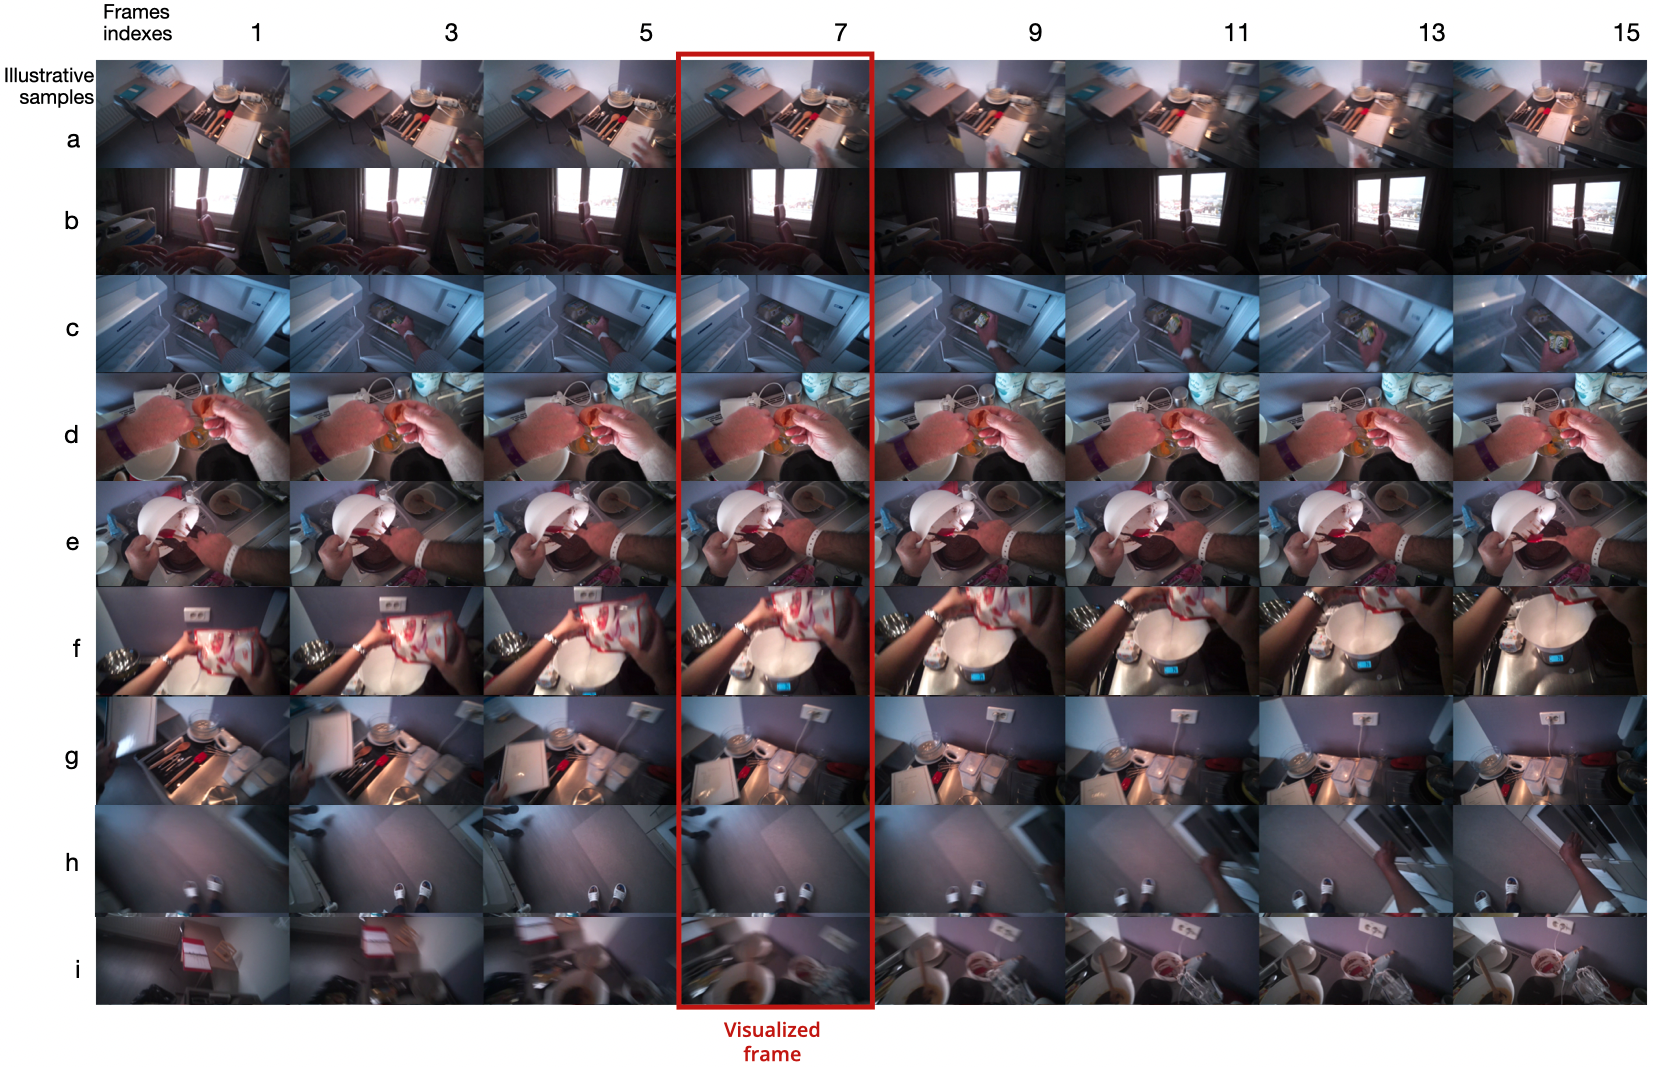
\includegraphics[width=0.9\linewidth]{figures/chapter_5_visual_probing.png}
    \caption{\textbf{Eight equally spaced frames within the encoder's temporal horizon (16 frames; $\approx 640$ms).} In most cases (rows a--e), visual appearance remains consistent, supporting the use of the central frame as a visual probe. However, rapid head or hand motion (rows f--i) can cause the central frame to inadequately represent the full action semantics. In practice, inspecting multiple independent central frames reveals consistent motion blur patterns, enabling reliable annotation.}
    \label{fig:supp_visual_probing_frames}
\end{figure}

\subsection{Prototype visual probe illustration}

\Cref{fig:supp_prototype_probe} illustrates the visual probe annotation image for consolidated prototypes.

\begin{figure}[!htbp]
    \centering
    \includegraphics[width=1.0\linewidth]{figures/prototype_visual_probe.png}
    \caption{\textbf{Illustration of a prototype visual probe.} Each item corresponds to the nearest-neighbors visual probe of a constituent centroid. In this example, the prototype is accepted, as all centroids consistently capture the action of ``pouring an ingredient''.}
    \label{fig:supp_prototype_probe}
\end{figure}

%==============================================================================
\section{Temporal segmentation evaluation}
\label{sec:supp_temporal_eval}
%==============================================================================

In the absence of fine-grained temporal annotations, we propose to evaluate the temporal segmentation qualitatively using participants' Gram matrices and via the impact of the majority voting scheme on the symbolic representation.

\subsection{Visual evaluation via Gram matrices}

\Cref{fig:supp_gram_cpts} shows detected change-points overlaid on Gram matrices for six participants, demonstrating that the segmentation accurately captures fine-grained action transitions corresponding to the smallest diagonal blocks.

\begin{figure}[!htbp]
    \centering
    \includegraphics[width=1.0\linewidth]{figures/gram_participant_cpts.png}
    \caption{\textbf{Gram matrices with detected change-points overlaid.} Vertical and horizontal lines indicate detected change-points. The segmentation accurately captures fine-grained action transitions, isolating small segments of similar pairwise cosine similarity. Notable events such as reading successive recipe pages are correctly identified. The ``harlequin'' patterns (green boxes) caused by the participant's hand intermittently entering the view are not isolated as distinct segments, illustrating the role of the minimum penalty heuristic in preventing over-segmentation.}
    \label{fig:supp_gram_cpts}
\end{figure}

\subsection{Effect of temporal smoothing}

\Cref{fig:supp_temporal_smoothing} illustrates the effect of segment-level majority voting on symbolic representations, showing how this step reduces spurious label fluctuations and yields more naturalistic and temporally coherent symbolic sequences.

\begin{figure}[!htbp]
    \centering
    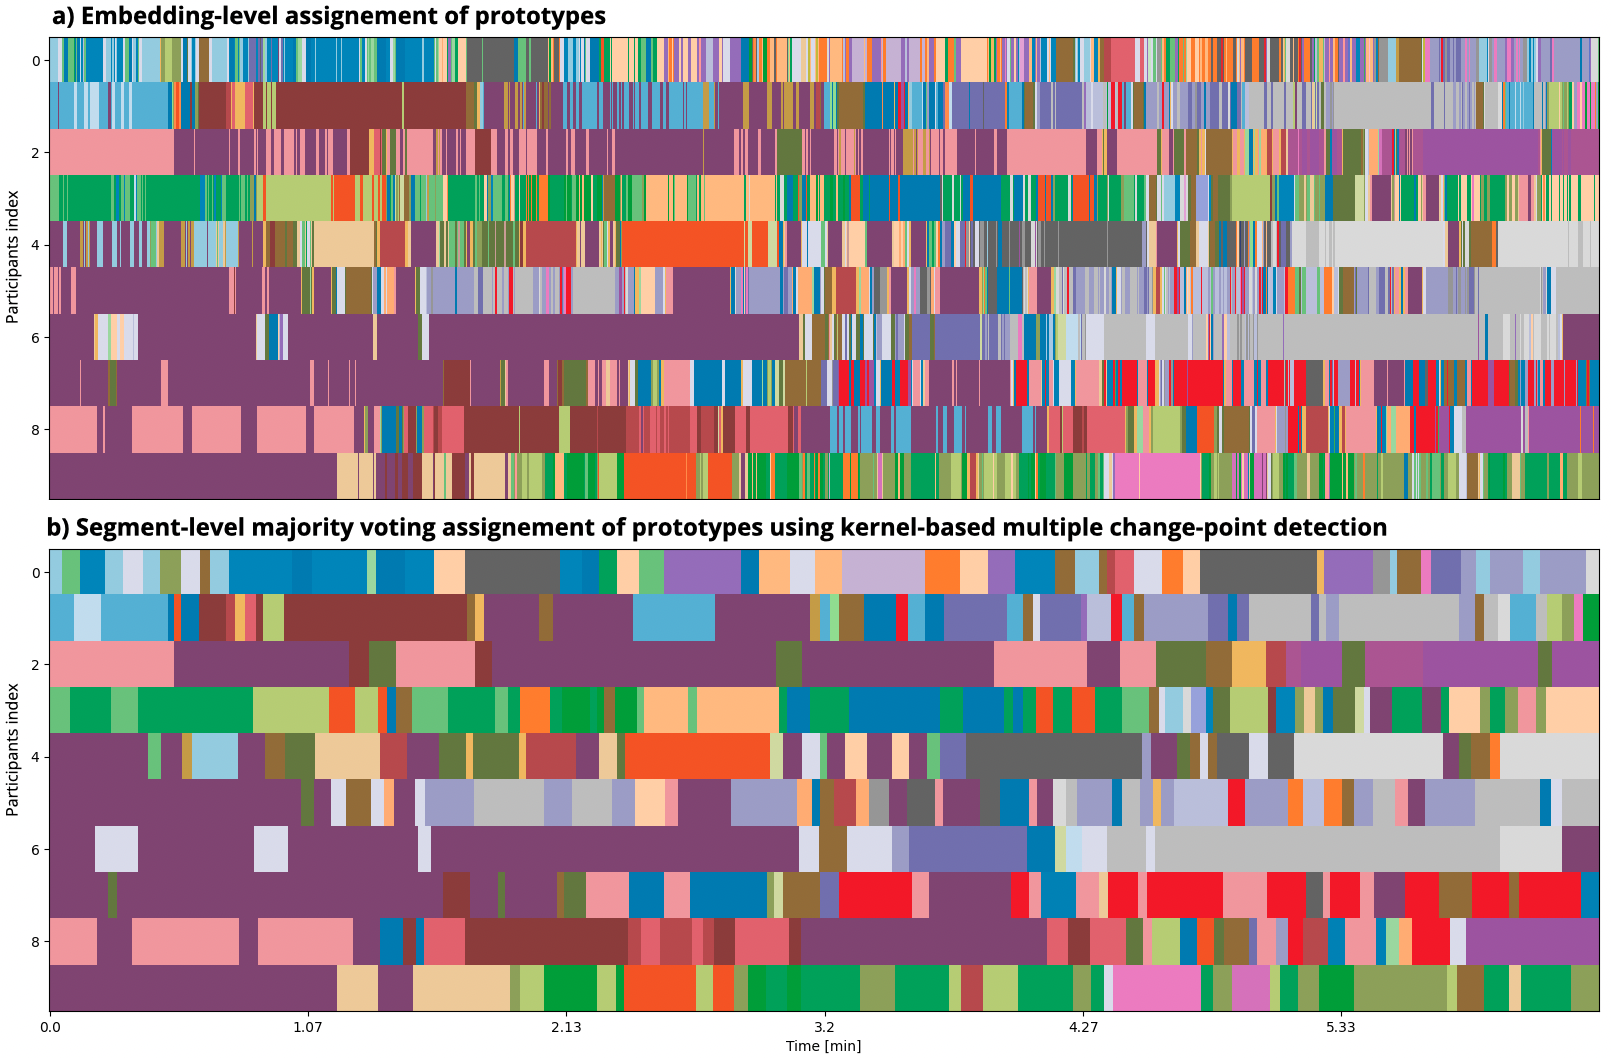
\includegraphics[width=0.9\linewidth]{figures/chapter_5_temporal_smoothing.png}
    \caption{\textbf{Effect of temporal smoothing on symbolic representations.} Symbolic sequences from 10 randomly sampled egocentric videos using (a) raw prototype assignments and (b) after applying unsupervised temporal action segmentation with segment-level majority voting. The smoothing step reduces noise and yields more temporally coherent prototype sequences.}
    \label{fig:supp_temporal_smoothing}
\end{figure}


\subsection{Detailed summary of the symbolization procedure experiments}

\begin{table}[!htbp]
    \centering
    \begin{tabular}{lcc}
        \toprule
        Stage & \texttt{Model-A} & \texttt{Model-B} \\
        \midrule
        Initial centroids ($p=8, C=100$) & 800 & 800 \\
        Valid centroids  & 642 & 613 \\
        $1^{st}$ HAC & 178 & 178 \\
        $2^{nd}$ HAC & 75 & 65 \\
        \midrule
        Accepted prototypes & 55 (72.3\%) & 45 (69.2\%) \\
        Rejected prototypes & 21 (27.7\%) & 20 (30.8\%) \\
        \midrule
        Background prop. (\%) & 15.7 $\pm$ 7.6 & 15.8 $\pm$ 7.7 \\
        Segment duration (s) & 8.357 $\pm$ 12.437 & 8.449 $\pm$ 12.878 \\
        $p^{\text{labels}}_{\text{change}}$ (\%) & 29.5 $\pm$ 3.8 & 28.0 $\pm$ 4.0 \\
        $p^{\text{withdrawn}}_{\text{CP}}$ (\%) & 21.5 $\pm$ 4.7 & 22.4 $\pm$ 5.2 \\
        $d_\text{tot}$ & 1856.5 $\pm$ 622.9 & 1840.3 $\pm$ 608.5 \\
        \bottomrule
    \end{tabular}
    \caption{\textbf{Prototype vocabulary estimation pipeline summary.} From initial centroid accumulation to final acceptance after redundancy reduction and manual inspection. $p^{\text{labels}}_{\text{change}}$: proportion of label switches between pointwise and segment-level assignments; $p^{\text{withdrawn}}_{\text{CP}}$: proportion of change-points between identical consecutive labels; $d_\text{tot}$: total sum of cosine assignment distances.}
    \label{tab:supp_pipeline}
\end{table}


%==============================================================================
\section{Additional assessments of the symbolic representations generalizability and fidelity}
\label{sec:supp_generalizability}
%==============================================================================

% \subsection{Generalizability to unseen participants}

% Prototype semantics are assessed using nearest-neighbor visual probes drawn from both training and held-out participants. \Cref{fig:chapter_5_visual_probes} shows that visual semantics remain stable across training and testing participants.

% \begin{figure}[!htbp]
%     \centering
%     \includegraphics[width=0.9\linewidth]{figures/chapter_5_visual_probes.png}
%     \caption{\textbf{Randomly selected visual probes of egocentric video prototypes.} Prototype generalizability to testing participants is assessed via nearest-neighbor visual probes (left and middle columns). Semantic consistency within prototypical regions is further examined in testing participants by comparing nearest- and furthest-neighbor visual probes (middle and right columns). Prototypes were randomly sampled from \texttt{Model-B}.}
%     \label{fig:chapter_5_visual_probes}
% \end{figure}

% \subsection{Within- and across-participant consistency}

% \Cref{fig:supp_subjects_rows} visualizes multiple occurrences of each prototype across participants, demonstrating consistent capture of the same underlying action both within and across individuals.

% \begin{figure}[!htbp]
%     \centering
%     \includegraphics[width=0.8\linewidth]{figures/chapter_5_subjects_rows.png}
%     \caption{\textbf{Illustrative examples of prototype assignments within and across participants.} For each prototype, up to ten segment occurrences are sampled across twenty participants. While occasional outliers are present, the majority of samples consistently capture similar actions across individuals, highlighting both the robustness and the semantic coherence of the prototype vocabulary.}
%     \label{fig:supp_subjects_rows}
% \end{figure}

\subsection{Additional visual probes}
%TODO: check this first apd: is correct 
We provide in \Cref{fig:supp_visual_probes_second} additional examples of nearest- and furthest-neighbors visual probes for randomly selected prototypes from \texttt{Model-B}, supporting the generalizability of the prototypes to unseen participants, as well as their semantic consistency within prototypical regions.

\begin{figure}[!htbp]
    \centering
    \includegraphics[width=0.9\linewidth]{figures/chapter_5_visual_probes_second.png}
        \caption{\textbf{Randomly selected visual probes of egocentric video prototypes.} We assess prototypes generalizability to testing participants via nearest-neighbors visual probes (left and middle columns). The semantic consistency within prototypical regions is assessed in testing participants by comparing nearest-neighbors and furthest-neighbors visual probes (middle and right columns).}
    \label{fig:supp_visual_probes_second}
\end{figure}

\subsection{Vocabulary exhaustivity via UMAP projection}

\Cref{fig:supp_umap} shows two-dimensional UMAP projections of prototypes and empirical samples, demonstrating that prototypes span the majority of the empirical data distribution.

\begin{figure}[!htbp]
    \centering
    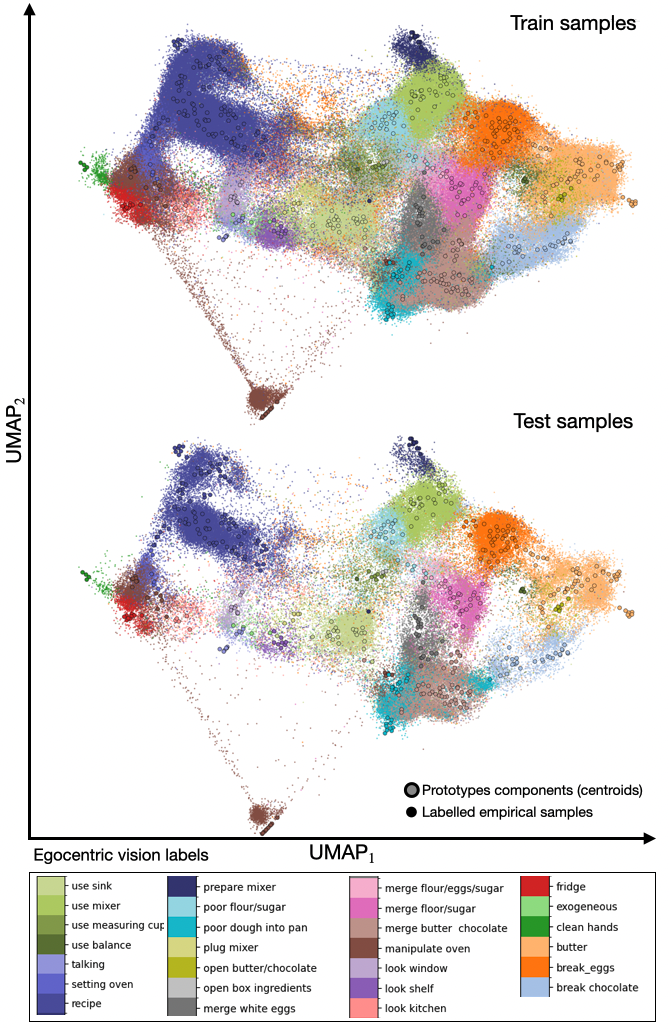
\includegraphics[width=0.9\linewidth]{figures/chapter_5_umap.png}
    \caption{\textbf{Two-dimensional UMAP projection of the prototype vocabulary centroids, training samples (top) and test samples (bottom).} The prototype vocabulary spans a substantial portion of the empirical training and testing samples, indicating broad coverage of participants' visual experience during the cooking task. This low-dimensional projection reveals the proximity between visually similar action classes (e.g., opening the fridge (red) and manipulating the oven (brown)) and temporally close actions (e.g., preparing the mixer (dark purple) and using it (light green)).}
    \label{fig:supp_umap}
\end{figure}

%==============================================================================
\section{Inter-rater reliability analysis}
\label{sec:supp_interrater}
%==============================================================================

To assess robustness to subjective annotation variability, we created two independent prototype models (\texttt{Model-A} and \texttt{Model-B}) based on annotations from different raters.

\subsection{Agreement quantification}

Inter-rater reliability was measured using Cohen's $\kappa$ on a shared set of 400 images. \Cref{tab:supp_interrater} summarizes the results.

\begin{table}[!htbp]
    \centering
    \begin{tabular}{l c}
    \toprule
    Grouping & $\kappa$ [95\% CI] \\
    \midrule
    Fine-grained (4 classes) & 0.46 [0.37, 0.55] \\
    Ambiguous vs Definitive  & 0.44 [0.35, 0.54] \\
    Task vs Exogenous        & 0.78 [0.57, 0.93] \\
    \bottomrule
    \end{tabular}
    \caption{\textbf{Inter-annotator agreement.} Cohen's $\kappa$ for different category grouping schemes. Annotators exhibit moderate agreement on quality labels but substantial agreement on the task/exogenous distinction.}
    \label{tab:supp_interrater}
\end{table}

These results indicate that while there is substantial concordance on the task/exogenous distinction, judgments about prototype quality are more subjective. Discrepancies mainly arose in clusters where experience with the procedure matters (e.g., some visually similar actions that cannot be disentangled by the encoder).


%==============================================================================
\section{Vocabulary comparison analysis}
\label{sec:supp_vocabulary_comparison}
%==============================================================================

\subsection{Embedding-level matching}

\Cref{fig:supp_assignment_cost} shows the embedding-level assignment cost matrix between the two vocabularies.

\begin{figure}[!htbp]
    \centering
    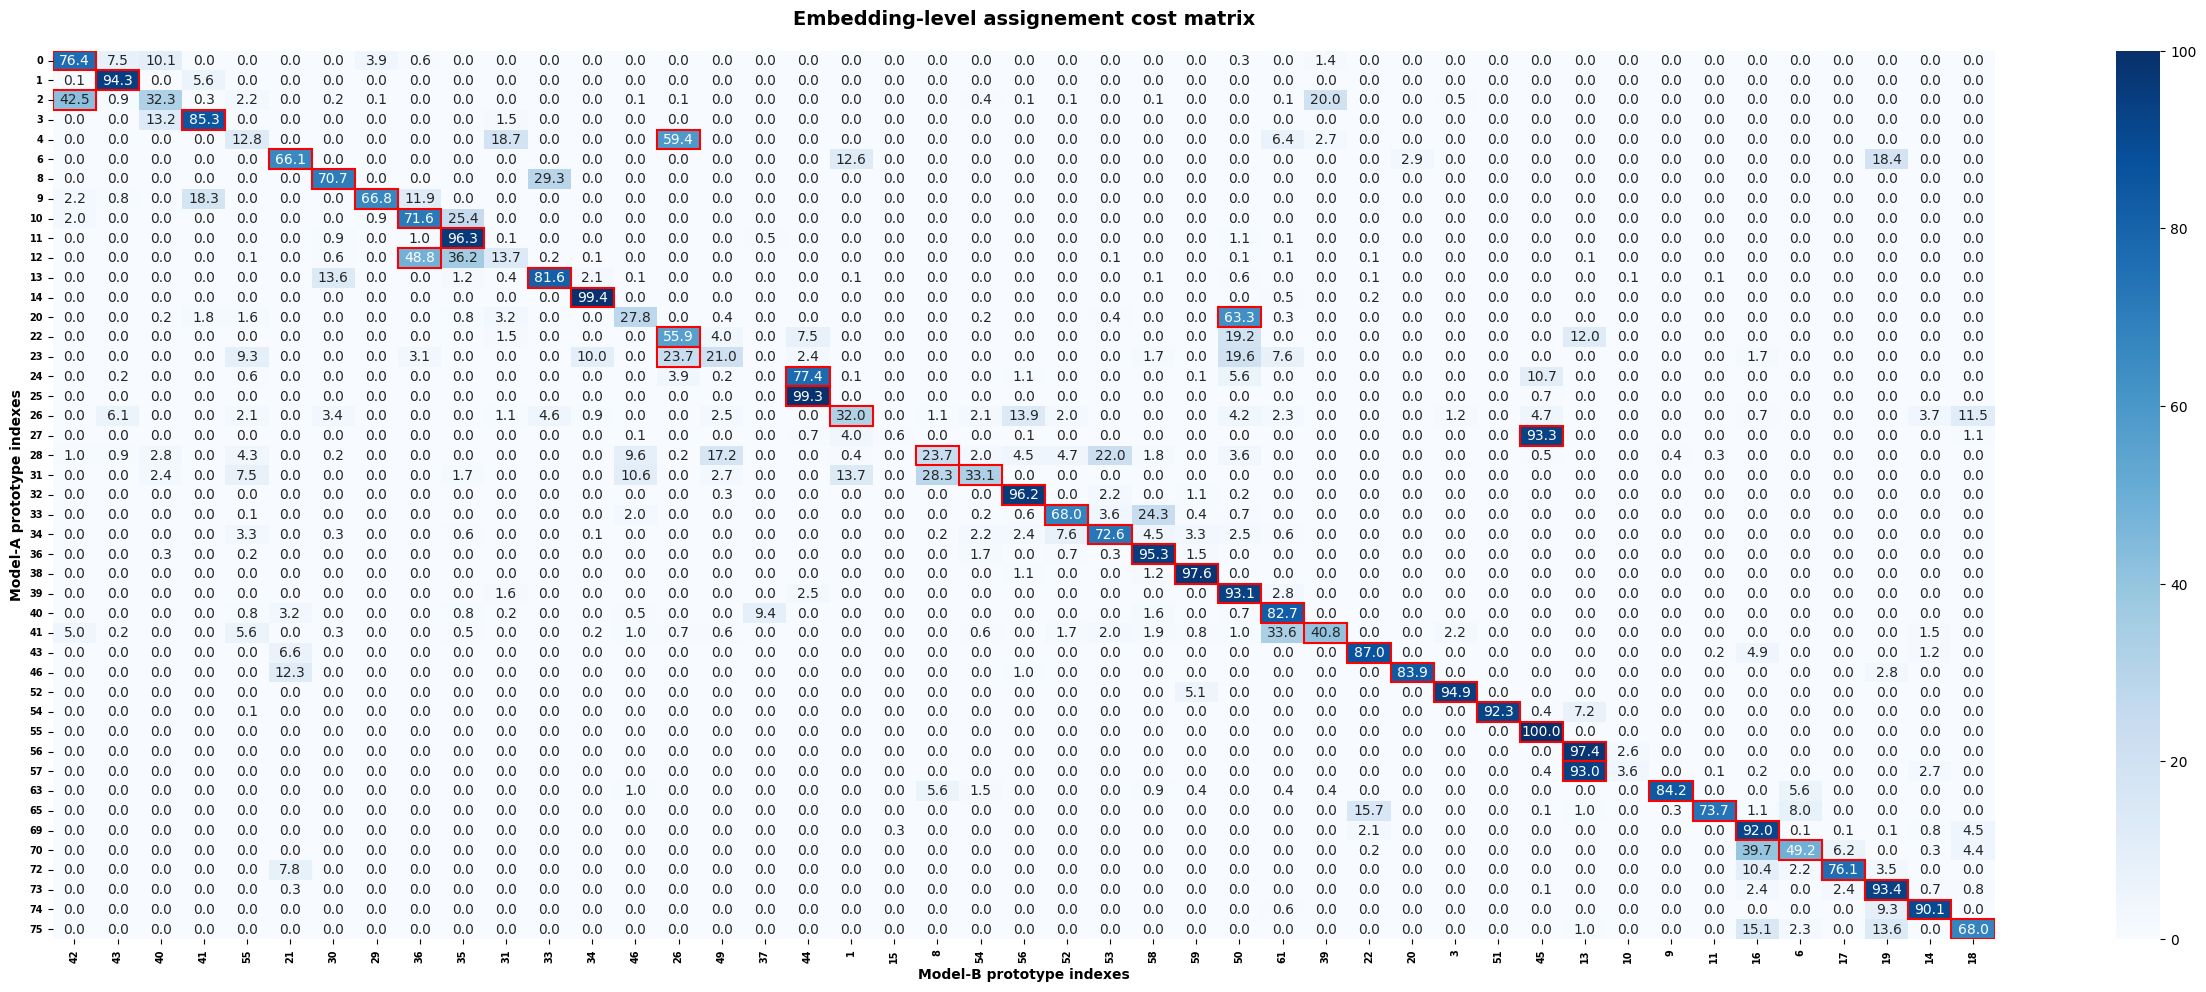
\includegraphics[width=1.0\linewidth]{figures/chapter_5_assignement_cost.png}
    \caption{\textbf{Embedding-level assignment cost matrix (row-normalized).} Each row represents a valid prototype from \texttt{Model-A}, each column from \texttt{Model-B}. Columns are ordered using Hungarian matching. Darker diagonal structures indicate sharp one-to-one correspondences, while spread-out rows highlight redundant prototypes.}
    \label{fig:supp_assignment_cost}
\end{figure}

The dominant diagonal structure indicates sharp one-to-one correspondences, with a few spread-out rows revealing redundant prototypes in both vocabularies. Exhaustive inspection of the matching prototypes was performed to assess the overlap and differences between the two vocabularies. Importantly, we did not find prototypes present in one vocabulary but entirely absent from the other, suggesting both vocabularies effectively capture a similar range of egocentric actions.

% \subsection{Top-k prototype matches}

% \Cref{fig:supp_matches} illustrates top-2 matches between prototypes, confirming semantic alignment despite vocabulary differences.

% \begin{figure}[!htbp]
%     \centering
%     \includegraphics[width=0.9\linewidth]{figures/chapter_5_matches.png}
%     \caption{\textbf{Top-2 prototype matches based on embedding overlap.} The anchor prototype from \texttt{Model-A} (left) is matched to its best (middle) and second-best (right) counterparts from \texttt{Model-B}. All three prototypes consistently capture ``merging the dough'', demonstrating semantic alignment while illustrating residual redundancies.}
%     \label{fig:supp_matches}
% \end{figure}

% \begin{figure}[!htbp]
%     \centering
%     \includegraphics[width=0.9\linewidth]{figures/chapter_5_matches_second_best.png}
%     \caption{\textbf{Additional examples of prototype matches.} Further examples showing top-2 matches between vocabularies.}
%     \label{fig:supp_matches_second}
% \end{figure}

% Importantly, we did not find prototypes present in one vocabulary but entirely absent from the other, suggesting both vocabularies effectively capture a similar range of egocentric actions.


% %==============================================================================
% \section{Symbolic Representation Comparison}
% \label{sec:supp_sr_comparison}
% %==============================================================================

% \subsection{Agreement metrics}

% Agreement between symbolic representations produced by both vocabularies was quantified using:
% \begin{itemize}
%     \item \textbf{Normalized Mutual Information (NMI):} 0.791 (95\% CI: [0.790, 0.792])
%     \item \textbf{Adjusted Rand Index (ARI):} 0.682 (95\% CI: [0.680, 0.685])
% \end{itemize}

% These values indicate strong semantic alignment despite vocabulary-level redundancy.

% \subsection{Temporal granularity comparison}

% \Cref{fig:supp_ecdf} compares the empirical cumulative density functions of segment durations across models.

% \begin{figure}[!htbp]
%     \centering
%     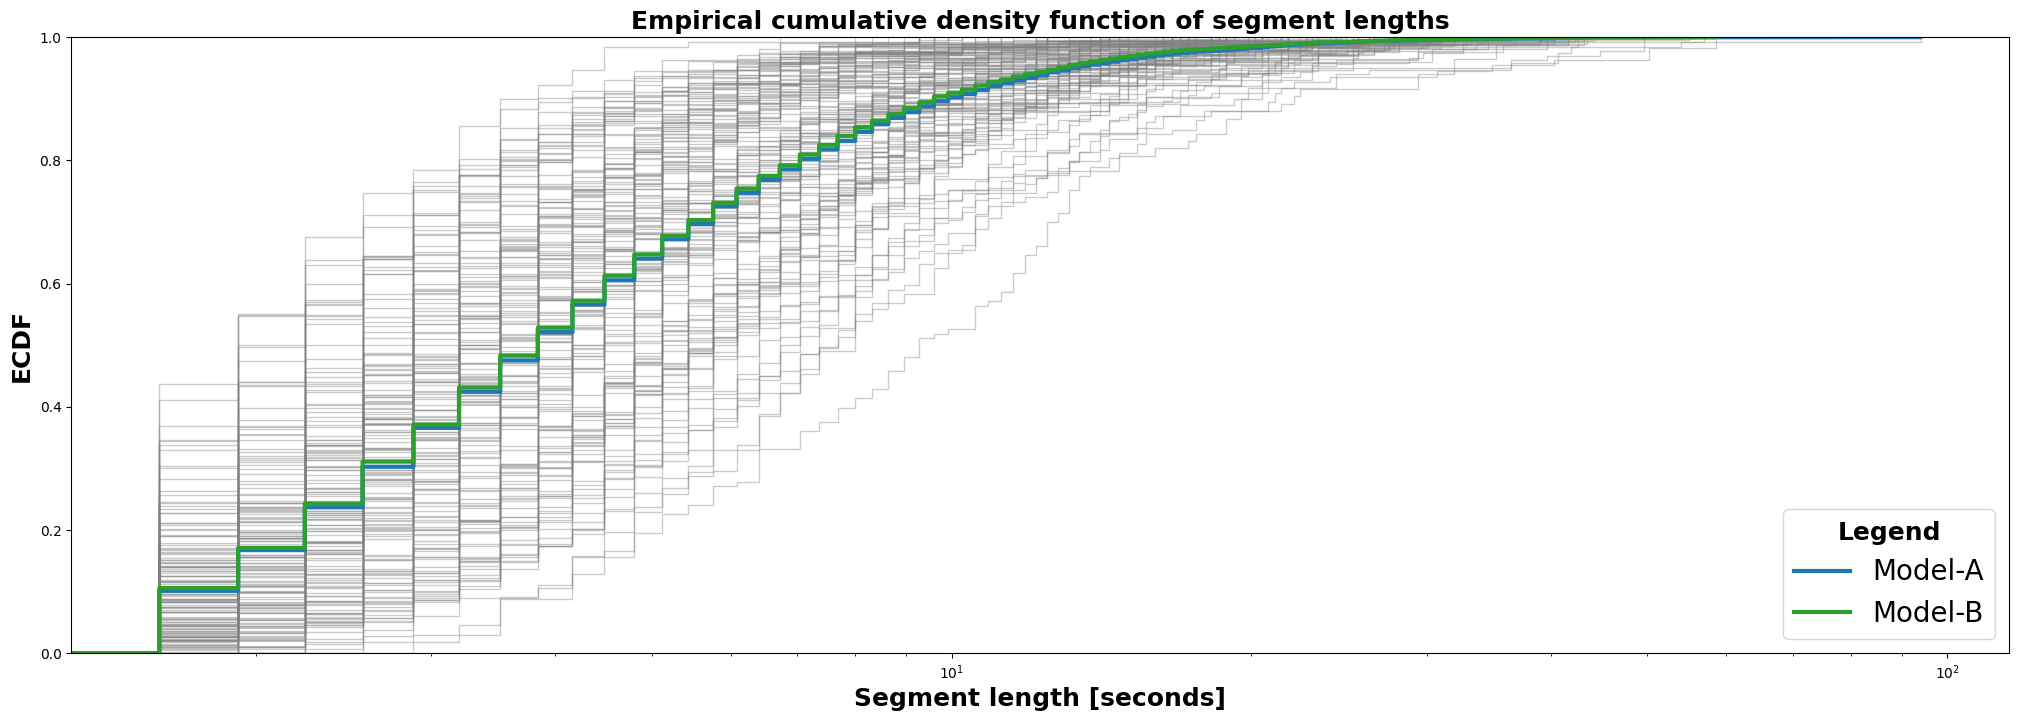
\includegraphics[width=0.9\linewidth]{figures/chapter_5_segments_duration_model_comparison.png}
%     \caption{\textbf{ECDF of segment durations.} Both models capture similar temporal dynamics granularity, with median durations of 6.4s (\texttt{Model-A}) and 6.6s (\texttt{Model-B}).}
%     \label{fig:supp_ecdf}
% \end{figure}

% Total segment counts were $1{,}247 \pm 290$ for \texttt{Model-A} and $1{,}298 \pm 310$ for \texttt{Model-B}, confirming similar temporal resolutions.

% \subsection{Background assignment consistency}

% \Cref{tab:supp_bg_confusion} shows the confusion matrix for background assignments.

% \begin{table}[!htbp]
%     \centering
%     \begin{tabular}{lcc}
%         \toprule
%         & \textbf{B: Non-background} & \textbf{B: Background} \\
%         \midrule
%         \textbf{A: Non-background} & 0.80 & 0.04 \\
%         \textbf{A: Background}     & 0.04 & 0.12 \\
%         \bottomrule
%     \end{tabular}
%     \caption{\textbf{Confusion matrix of background assignments.} Agreement between \texttt{Model-A} (rows) and \texttt{Model-B} (columns). Both models agree on 92\% of embeddings.}
%     \label{tab:supp_bg_confusion}
% \end{table}

% The ARI (0.627, 95\% CI: [0.625, 0.630]) and NMI (0.431, 95\% CI: [0.428, 0.434]) for background detection indicate moderate concordance, suggesting that despite general overlap, the vocabularies may differ in identifying low-confidence assignments.

% \subsection{Final symbolic representations}

% \Cref{fig:supp_final_sr} visualizes the final symbolic representations for all participants.

% \begin{figure}[!htbp]
%     \centering
%     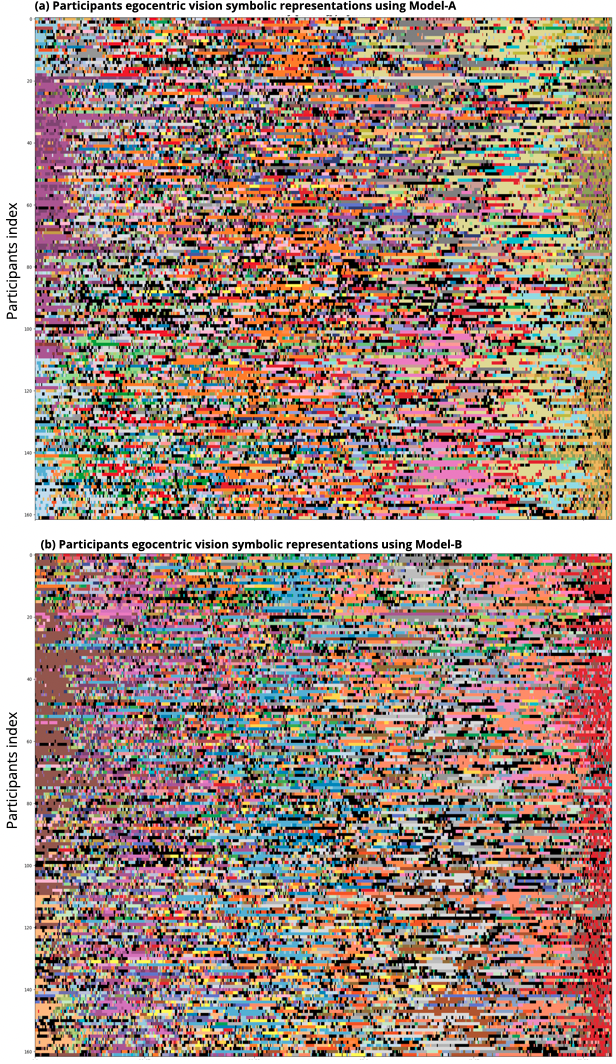
\includegraphics[width=0.8\linewidth]{figures/chapter_5_final_symbolic_representation.png}
%     \caption{\textbf{Symbolic representations using \texttt{Model-A} (a) and \texttt{Model-B} (b).} Each row corresponds to a participant, each color to a prototype. Color-coding is independent for each model. Sequences are upsampled for visualization.}
%     \label{fig:supp_final_sr}
% \end{figure}

%==============================================================================
\section{Clinical analysis: statistical methods and tables}
\label{sec:supp_clinical_tables}
%==============================================================================

\subsection{Fragmentation rate comparisons}

\begin{table}[!htbp]
\centering
\begin{tabular}{l l r r r r r r r}
\hline
Group 1 & Group 2 & $U$ & $p$ & $r_{rb}$ & Med. 1 & Med. 2 & $n_1$ & $n_2$ \\
\hline
\multicolumn{9}{c}{\textbf{Binary group distinction}} \\
\hline
Control & Patients & 1765.0 & $1.24 \times 10^{-3}$ & -0.414 & 6.0 & 4.9 & 26 & 96 \\
\hline
\multicolumn{9}{c}{\textbf{Subgroup analysis}} \\
\hline
Control & RIL & 760.0  & $1.01 \times 10^{-4}$ & -0.580 & 6.0 & 4.3 & 26 & 37 \\
Control & TBI & 1005.0 & $2.35 \times 10^{-2}$ & -0.310 & 6.0 & 5.2 & 26 & 59 \\
RIL     & TBI & 771.0  & $1.60 \times 10^{-2}$ &  0.294 & 4.3 & 5.2 & 37 & 59 \\
\hline
\end{tabular}
\caption{\textbf{Pairwise comparisons of fragmentation rate across groups.} $U$ = Mann-Whitney statistic, $p$ = p-value, $r_{rb}$ = rank-biserial effect size. Medians indicate the central tendency of fragmentation rate per group (transitions per minute). TBI: traumatic brain injury; RIL: radiation-induced leukoencephalopathy. Significance level was set at $p<0.05$.}
\label{tab:fragmentation_results}
\end{table}

\subsection{Analysis of exogenous and task-related actions}

\begin{table}[!htbp]
\centering
\begin{tabular}{l l r r r r r r r}
\hline
Group 1 & Group 2 & $U$ & $p$ & $r_{rb}$ & Med. 1 & Med. 2 & $n_1$ & $n_2$ \\
\hline
\multicolumn{9}{c}{\textbf{Binary group distinction}} \\
\hline
Control & Patients & 1030.5 & $1.75 \times 10^{-1}$ &  0.174 & 0.083 & 0.11 & 26 & 96 \\
\hline
\multicolumn{9}{c}{\textbf{Subgroup analysis}} \\
\hline
Control & RIL & 291.0  & $8.15 \times 10^{-3}$ &  0.395 & 0.083 & 0.17 & 26 & 37 \\
Control & TBI & 739.5  & $7.97 \times 10^{-1}$ &  0.036 & 0.083 & 0.091 & 26 & 59 \\
RIL     & TBI & 1499.0 & $2.18 \times 10^{-3}$ & -0.373 & 0.17  & 0.091 & 37 & 59 \\
\hline
\end{tabular}
\caption{\textbf{Pairwise comparisons in the proportion of exogenous segments across groups.} $U$ = Mann-Whitney statistic, $p$ = p-value, $r_{rb}$ = rank-biserial effect size. Medians indicate the central tendency of the proportion of exogenous actions per group. TBI: traumatic brain injury; RIL: radiation-induced leukoencephalopathy. Significance level was set at $p<0.05$.}
\label{tab:task_exo_results}
\end{table}



% %==============================================================================
% \section{Clustering implementation comparison}
% \label{sec:supp_clustering_comparison}
% %==============================================================================

% We compared $k$-means implementations from Faiss \cite{douze2024faiss} and Scikit-learn \cite{sklearn} using both cosine and Euclidean distance metrics. \Cref{tab:supp_clustering_comparison} reports the number of valid (semantically unequivocal) and ambiguous centroids for $C=100$ clusters in the first iteration.

% \begin{table}[!htbp]
%     \centering
%     \begin{tabular}{lcc|cc}
%         \toprule
%         \multirow{2}{*}{\textbf{Category}} &
%         \multicolumn{2}{c|}{\textbf{Cosine}} &
%         \multicolumn{2}{c}{\textbf{Euclidean}} \\
%         & \textbf{Faiss} & \textbf{Scikit-Learn} & \textbf{Faiss} & \textbf{Scikit-Learn} \\
%         \midrule
%         Valid & 75 & 69 & 68 & 54 \\
%         Ambiguous & 25 & 31 & 32 & 46 \\
%         \bottomrule
%     \end{tabular}
%     \caption{\textbf{Number of valid and ambiguous centroids across implementations and distance metrics} ($C=100$, first iteration). Faiss with cosine distance yields the highest proportion of semantically unequivocal clusters.}
%     \label{tab:supp_clustering_comparison}
% \end{table}

% Faiss consistently outperforms Scikit-learn regardless of distance metric, and cosine distance outperforms Euclidean distance in both implementations. These results support our choice of Faiss with cosine distance for the centroid accumulation procedure.


% %==============================================================================
\section{Per-category composition analysis across diagnosis groups}
\label{sec:supp_per_category}
%==============================================================================

We present in \Cref{fig:supp_per_label_pathologie} the complete per-category comparison of symbolic representation composition across diagnosis groups. For each of the 28 action categories, we computed three metrics: number of occurrences, mean segment duration, and proportion of total task time. Pairwise group comparisons were performed using Mann--Whitney U tests with Benjamini--Hochberg correction for multiple comparisons. Significant differences ($p<0.05$) are indicated by brackets with annotated p-values.

\begin{figure}[!htbp]
    \centering
    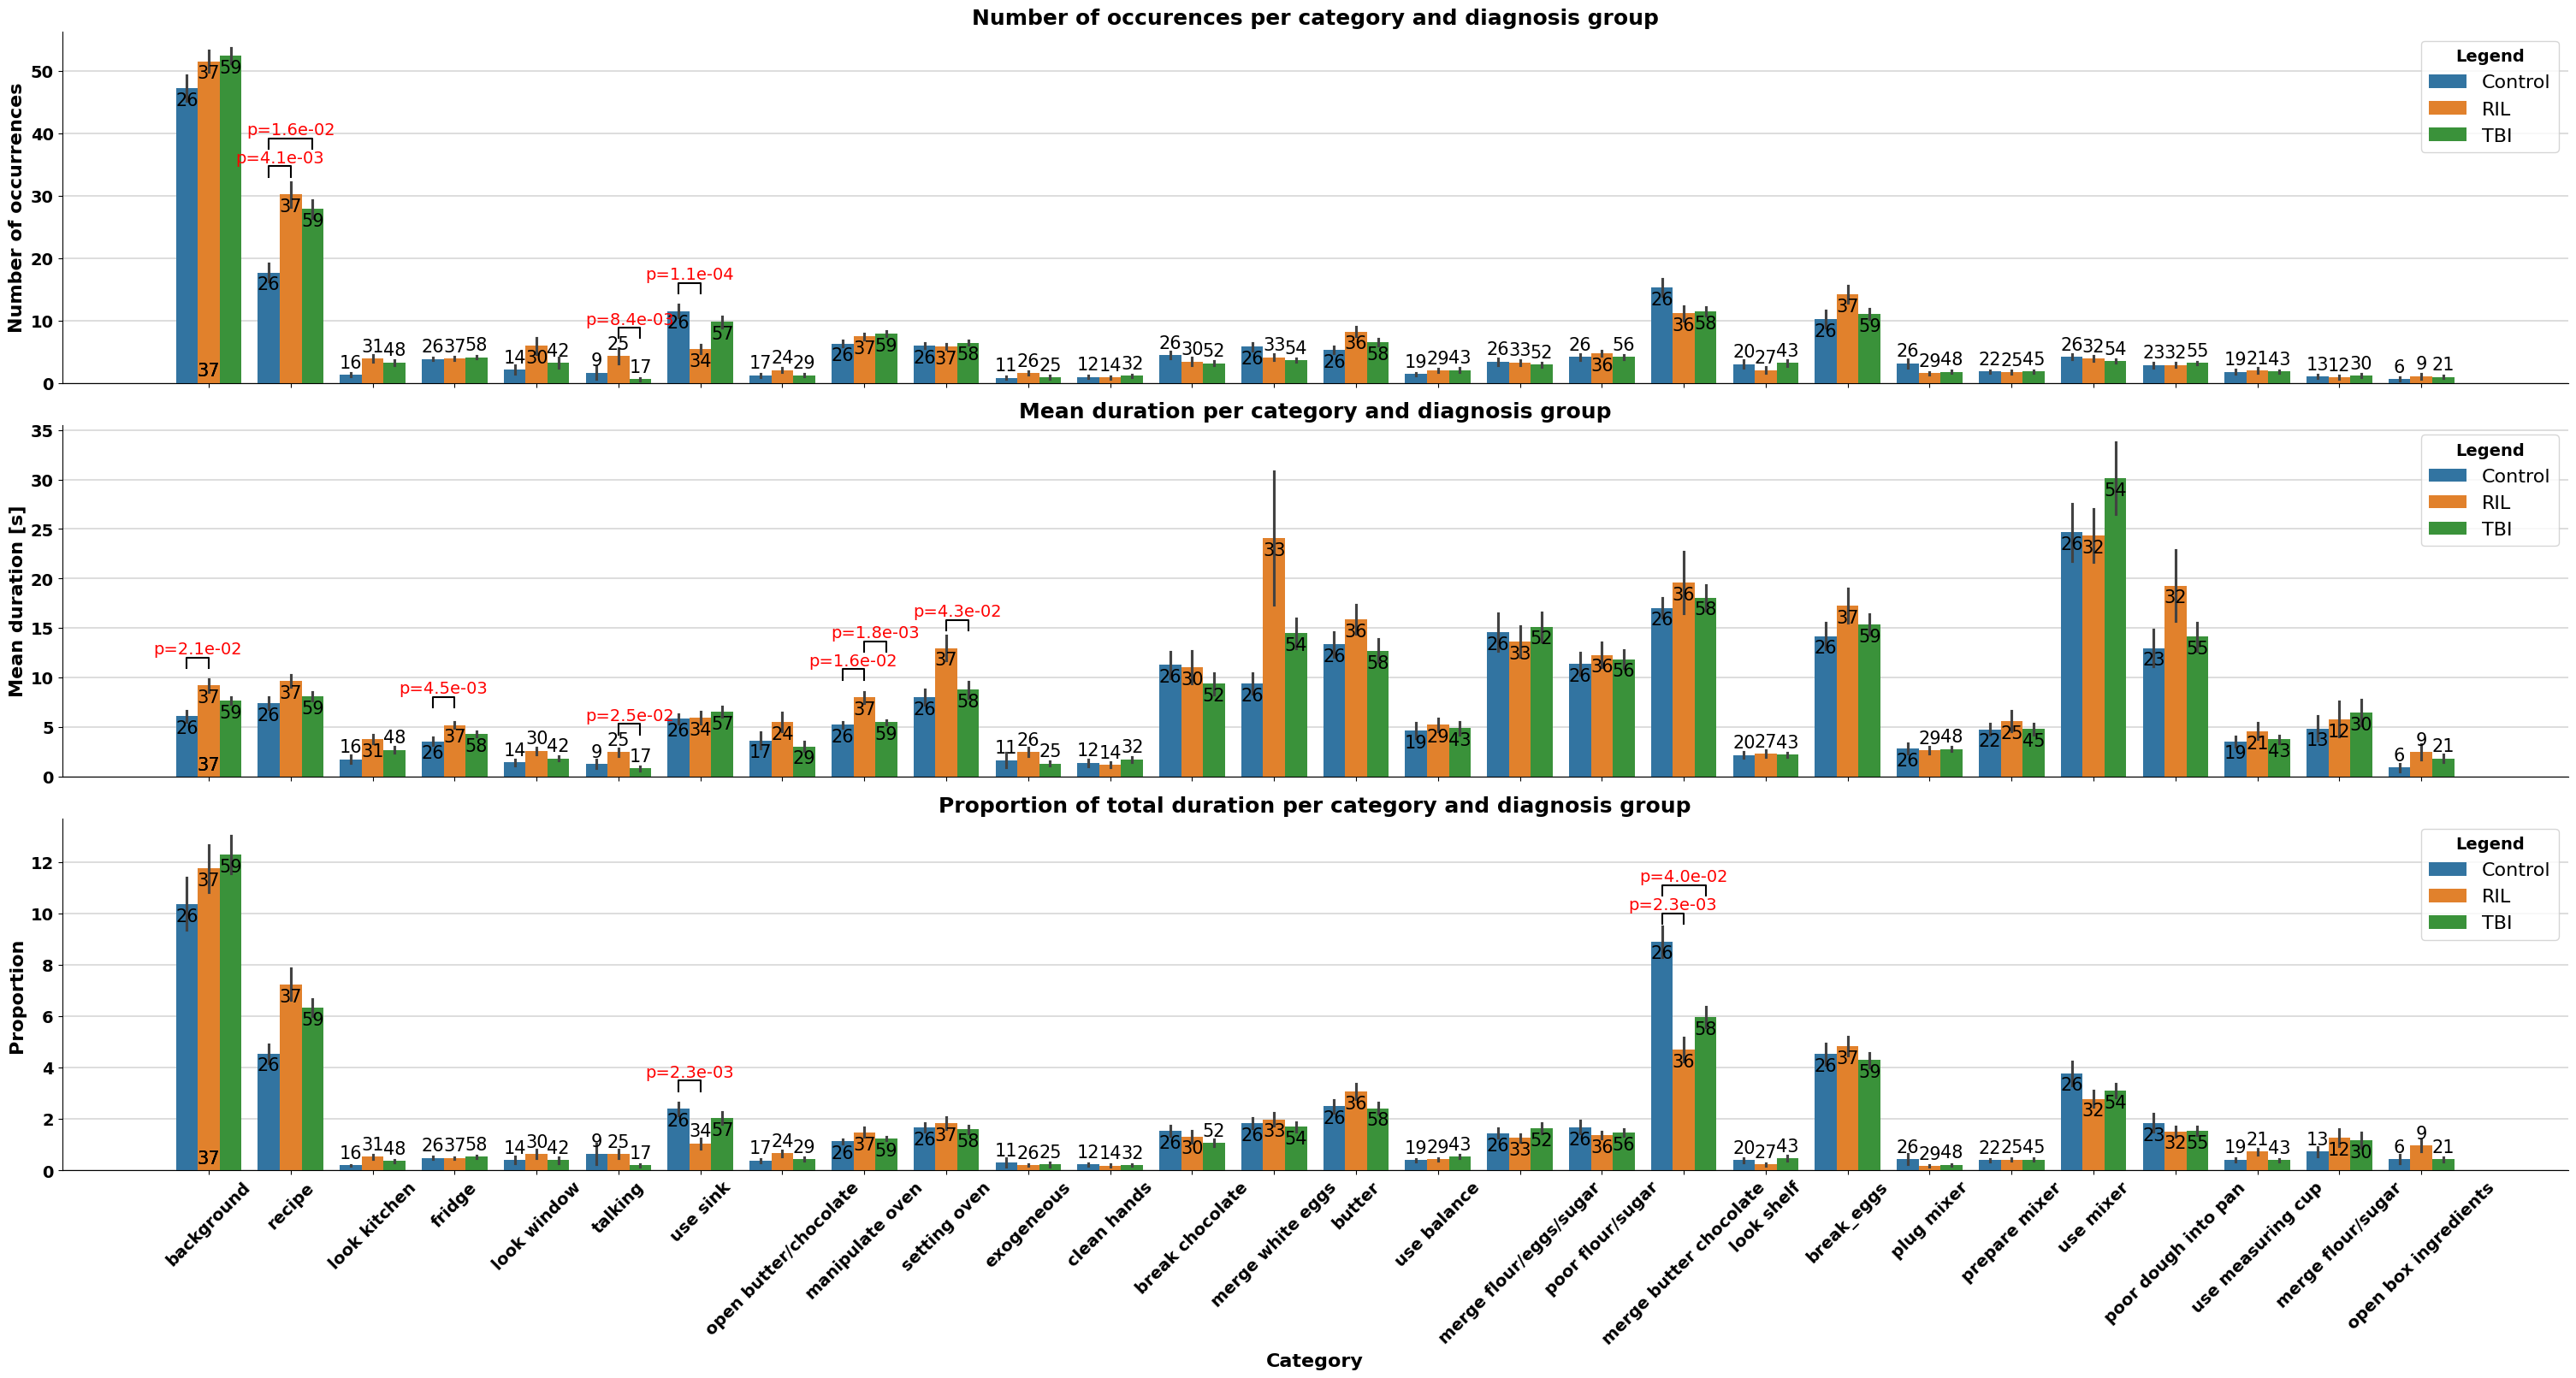
\includegraphics[width=1.0\textwidth]{figures/per_label_pathologie_p_values.png}
    \caption{\textbf{Comparison of number of occurrences (top), mean duration (middle), and proportion of time (bottom) of each action category across diagnosis groups.} Bars indicate mean values per category and group, with error bars representing standard error of the mean. Pairwise group differences within each category were tested using Mann--Whitney U tests with Benjamini--Hochberg correction, and significant differences are shown by brackets connecting the bars with annotated p-values. Statistical significance was set at $p<0.05$. TBI: traumatic brain injury; RIL: radiation-induced leukoencephalopathy.}
    \label{fig:supp_per_label_pathologie}
\end{figure}

%==============================================================================
\subsection{Statistical Methods}
\label{sec:supp_statistical_methods}
%==============================================================================

Pairwise group comparisons of fragmentation rate, number of occurrences, mean duration, and proportion of time in each category were performed using the non-parametric Mann--Whitney U test, with rank-biserial correlation estimating effect sizes. We corrected for false discovery rate inflation due to multiple comparisons by applying the Bonferroni-Hochberg procedure separately for each metric.

To quantify uncertainty around the aggregated empirical cumulative distribution functions (ECDFs), we computed $95\%$ confidence intervals via bootstrapping: repeated resampling with replacement of the observed segment durations yields a distribution of ECDF values at each duration, from which the $2.5^{\text{th}}$ and $97.5^{\text{th}}$ percentiles define the confidence bands.

Group differences in segment lengths were assessed using a linear mixed-effects model with participant as a random intercept and diagnosis group as a fixed effect. Model comparison was performed via a likelihood-ratio test between the null model (no group effect) and the alternative model (including group) using maximum likelihood estimation. Segment durations were log-transformed to reduce skewness, and fixed-effect estimates were back-transformed to the original scale to report multiplicative changes. This approach accounts for the non-independence of segments within participants and is recommended for hierarchical repeated-measures data \cite{Gelman2006,BAAYEN2008390}.

Statistics were calculated in Python V.3.10.16, using SciPy low-level functions V.1.10.1, and Statsmodels V.0.14.4.


\bibliographystyle{splncs04}
\bibliography{bibliography}

\end{document}
